% =====================================================================
% SOICT 2026 poster — A0 portrait (841 x 1189 mm)
% Paper: papers/soict2026/manuscript/main.tex (camera-ready, paper 3215)
% Build: ./compile.sh  (XeLaTeX). Every number comes from the paper.
% =====================================================================
\documentclass{article}
\usepackage[paperwidth=841mm, paperheight=1189mm, margin=0mm]{geometry}
\usepackage{fontspec}
\usepackage{graphicx}
\usepackage{booktabs}
\usepackage{array}
\usepackage{xcolor}
\usepackage{tikz}
\usetikzlibrary{positioning, arrows.meta, fit, backgrounds, calc}
% tcolorbox 2024+ calls LaTeX tagging hooks that the BasicTeX 2024 kernel
% lacks; no-op stand-ins keep the boxes working (they do nothing untagged).
\providecommand\UseTaggingSocket[1]{}
\providecommand\SuspendTagging[1]{}
\providecommand\ResumeTagging[1]{}
\usepackage[most]{tcolorbox}
\usepackage{qrcode}
\usepackage{enumitem}
\usepackage{amssymb}
\usepackage{adjustbox}

\IfFontExistsTF{Helvetica Neue}
  {\setmainfont{Helvetica Neue}[Ligatures=TeX]}
  {\IfFontExistsTF{TeX Gyre Heros}{\setmainfont{TeX Gyre Heros}[Ligatures=TeX]}{}}

\definecolor{accBlue}{HTML}{0072B2}
\definecolor{accGreen}{HTML}{009E73}
\definecolor{accOrange}{HTML}{D55E00}
\definecolor{accRed}{HTML}{C1121F}
\definecolor{inkDark}{HTML}{23373B}
\definecolor{paper}{HTML}{F6F8FA}
% Headline-number cards take the four affiliation logos' main colours, in
% the logos' left-to-right order (sampled from img/logo_*.png).
\definecolor{utcNavy}{HTML}{2A1258}
\definecolor{utcYellow}{HTML}{D4AA00}  % UTC logo yellow F0CC00, darkened for white (2.2:1 vs 1.57:1)
\definecolor{vnuBlue}{HTML}{2490CC}
\definecolor{uitBlue}{HTML}{2460FC}
\definecolor{nluGreen}{HTML}{00903C}
% Conclusion box: the organiser's (SoICT-HUST) red, sampled from img/org_soict_hust.png.
\definecolor{hustRed}{HTML}{BA1B2B}

\newcommand{\key}[1]{\textbf{\textcolor{accBlue}{#1}}}
\newcommand{\good}[1]{\textbf{\textcolor{accGreen!80!black}{#1}}}
\newcommand{\bad}[1]{\textbf{\textcolor{accRed}{#1}}}

\graphicspath{{../../papers/soict2026/manuscript/figures/}{img/}}

% Body text: 30 pt reads from about 1.5 m; tables and captions a step down.
\newcommand{\bodysize}{\fontsize{28}{34}\selectfont}
\newcommand{\tabsize}{\fontsize{26}{31}\selectfont}
\newcommand{\capsize}{\fontsize{21}{25}\selectfont}

\setlist[itemize]{leftmargin=1.1em, itemsep=0.15em, topsep=0.3em, label={\textcolor{accBlue}{\raisebox{0.12ex}{\scalebox{0.7}{$\blacksquare$}}}}}
\setlist[enumerate]{leftmargin=1.4em, itemsep=0.15em, topsep=0.3em, label={\textbf{\textcolor{accBlue}{\arabic*.}}}}

\newtcolorbox{sect}[2][]{enhanced, colback=white, colframe=accBlue,
  boxrule=1.4mm, arc=4mm, left=6mm, right=6mm, top=3.5mm, bottom=3.5mm,
  fonttitle=\fontsize{36}{42}\selectfont\bfseries, coltitle=white,
  colbacktitle=accBlue, toptitle=2mm, bottomtitle=2mm,
  title={#2}, before skip=0mm, after skip=0mm, halign=flush left, #1}

\newtcolorbox{takeaway}{enhanced, colback=accGreen!10, colframe=accGreen!70!black,
  boxrule=1.2mm, arc=3mm, left=6mm, right=6mm, top=2.5mm, bottom=2.5mm,
  before skip=5mm, after skip=0mm, halign=flush left}

\setlength{\parindent}{0pt}
\setlength{\tabcolsep}{10pt}
\pagestyle{empty}

\begin{document}
\special{pdf:docinfo<< /Title (A Distributed Real-Time Intrusion Detection System on a Jetson Orin Nano Super Edge Cluster using Kafka and PySpark -- SOICT 2026 poster) /Author (Thai Nguyen Vu, Bui Van Dung, Tri Nhut Do, Van Du Nguyen) >>}
% Posters read better ragged-right and unhyphenated: justified narrow
% columns produced split words ("ver-dict") and stretched gaps.
\raggedright\hyphenpenalty=10000\exhyphenpenalty=10000
\bodysize
\pagecolor{paper}

% =====================================================================
% HEADER
% =====================================================================
\newsavebox\topPart
\setbox\topPart=\vbox{\hsize=841mm
\noindent\begin{tikzpicture}[remember picture, overlay]
  \fill[accBlue] (current page.north west) rectangle ([yshift=-178mm]current page.north east);
  \fill[accRed] ([yshift=-178mm]current page.north west) rectangle ([yshift=-182mm]current page.north east);
  % Footer: conference line and the organisers' logos, kept apart from the
  % authors' affiliation logos in the header.
  \fill[accBlue] (current page.south west) rectangle ([yshift=52mm]current page.south east);
  \fill[accRed] ([yshift=52mm]current page.south west) rectangle ([yshift=56mm]current page.south east);
  \node[anchor=west, text=white, align=left, font=\fontsize{24}{30}\selectfont]
    at ([xshift=30mm, yshift=26mm]current page.south west)
    {\textbf{SOICT 2026} --- The 15th International Symposium on Information\\
     and Communication Technology \,·\, Ho Chi Minh City, Vietnam \,·\, 4--5 December 2026};
  \node[anchor=east, fill=white, rounded corners=4mm, inner xsep=6mm, inner ysep=4mm,
        font=\fontsize{19}{23}\selectfont, text=inkDark]
    at ([xshift=-30mm, yshift=26mm]current page.south east)
    {\begin{tabular}{@{}c@{}}Organized by\\[2mm]
\includegraphics[height=30mm]{org_soict_hust.png}\end{tabular}%
     \hspace{8mm}%
     \begin{tabular}{@{}c@{}}Co-organized by\\[2mm]
\includegraphics[height=30mm]{org_hcmus.png}\end{tabular}};
\end{tikzpicture}%
\vspace*{14mm}

\hspace*{30mm}%
\begin{minipage}[t]{655mm}
  \color{white}
  {\fontsize{60}{70}\selectfont\bfseries\raggedright\hyphenpenalty=10000 A Distributed Real-Time Intrusion Detection System
   on a Jetson Orin Nano Super Edge Cluster using Kafka and PySpark\par}
  \vspace{7mm}
  {\fontsize{38}{46}\selectfont \textbf{Thai Nguyen Vu}\textsuperscript{1} \quad Bui Van Dung\textsuperscript{2,3} \quad
   Tri Nhut Do\textsuperscript{2,3} \quad Van Du Nguyen\textsuperscript{4}\par}
  \vspace{5mm}
  \begin{minipage}[c]{405mm}
  {\fontsize{22}{29}\selectfont\raggedright
   \textsuperscript{1}Campus in Ho Chi Minh City, University of Transport and Communications, Ho Chi Minh City, Vietnam\\
   \textsuperscript{2}Vietnam National University, Ho Chi Minh City, Vietnam\\
   \textsuperscript{3}University of Information Technology, Ho Chi Minh City, Vietnam\\
   \textsuperscript{4}Faculty of Information Technology, Nong Lam University, Ho Chi Minh City, Vietnam\par}
  \end{minipage}%
  \hfill
  % Affiliation logos in affiliation order, on one white card so each reads
  % against its own (white) background.
  \begin{tikzpicture}[baseline=(card.center)]
    \node[fill=white, rounded corners=4mm, inner xsep=6mm, inner ysep=5mm] (card) {%
      
\includegraphics[height=36mm]{logo_utc.png}\hspace{7mm}%
      
\includegraphics[height=34mm]{logo_vnuhcm.png}\hspace{7mm}%
      
\includegraphics[height=34mm]{logo_uit.png}\hspace{7mm}%
      
\includegraphics[height=36mm]{logo_nlu.png}};
  \end{tikzpicture}%
\end{minipage}%
\hfill
\begin{minipage}[t]{115mm}
  \centering\color{white}
  {\fontsize{34}{40}\selectfont\bfseries SOICT 2026\par}
  \vspace{6mm}
  \colorbox{white}{\color{black}\qrcode[height=78mm]{https://github.com/vuthainguyen1602/Thesis_IDS}}\par
  \vspace{3mm}
  {\fontsize{20}{24}\selectfont Code \& configurations\par}
\end{minipage}%
\hspace*{30mm}

\vspace{10mm}

% =====================================================================
% KEY NUMBERS
% =====================================================================
\newcommand{\kpi}[3]{%
  \begin{tcolorbox}[enhanced, width=184mm, height=58mm, valign=center, halign=center,
    colback=white, colframe=#3, boxrule=2mm, arc=6mm, left=4mm, right=4mm, nobeforeafter, box align=top]
    {\fontsize{66}{72}\selectfont\bfseries\textcolor{#3}{#1}\par}
    \vspace{2mm}
    {\fontsize{22}{27}\selectfont #2\par}
  \end{tcolorbox}}
% Filled variant {number}{caption}{background}{number colour}: the caption
% turns white, so a light number colour (UTC yellow on UTC navy) reads well.
\newcommand{\kpifilled}[4]{%
  \begin{tcolorbox}[enhanced, width=184mm, height=58mm, valign=center, halign=center,
    colback=#3, colframe=#3, boxrule=2mm, arc=6mm, left=4mm, right=4mm, nobeforeafter, box align=top]
    {\fontsize{66}{72}\selectfont\bfseries\textcolor{#4}{#1}\par}
    \vspace{2mm}
    {\fontsize{22}{27}\selectfont\color{white}#2\par}
  \end{tcolorbox}}
\hspace*{30mm}%
\kpi{22.4}{flows/s sustained by pipeline split\\≈9× a single node (2.5)}{utcYellow}\hspace{8mm}%
\kpi{0.60\,J}{per verdict on two boards\\vs.\ 3.04\,J on a single node}{vnuBlue}\hspace{8mm}%
\kpi{69.5\%}{recall at 100\% precision\\every miss is a gate skip}{uitBlue}\hspace{8mm}%
\kpi{≈7{,}200×}{ONNX Runtime vs.\ PySpark, batch 10\\same forest, same predictions}{nluGreen}%

\vspace{9mm}

% =====================================================================
% TWO COLUMNS
% =====================================================================
}
\typeout{POSTER textheight=\the\textheight\space topskip=\the\topskip\space baselineskip=\the\baselineskip}\typeout{POSTER top=\the\dimexpr\ht\topPart+\dp\topPart\relax}
\noindent\box\topPart\par
% Both columns get the same fixed height and spread their boxes with \vfill,
% so their bottoms line up. Keep \colheight above the taller column's natural
% height (see the POSTER line in the log) and below 1189 mm minus the header.
\newlength\colheight\setlength\colheight{905mm}
\newsavebox\colL\newsavebox\colR
\begin{lrbox}{\colL}%
\begin{minipage}[t][\colheight][t]{381mm}\vspace{0pt}% top-align both columns
% ---------------------------------------------------------------------
\begin{sect}{Problem: three open gaps}
  Detectors now fit on single-board hardware, but a monolithic one classifies
  \key{every} flow and saturates an 8\,GB ARM board.
  \begin{enumerate}
    \item Recent edge IDS are measured on a \bad{single device}: what does a
          second board actually buy?
    \item Throughput, latency percentiles and \bad{energy} are rarely reported
          together for one deployed system.
    \item Offline scores can be inflated by \bad{leaky protocols} before the
          model is ever deployed.
  \end{enumerate}
  \begin{takeaway}
    \textbf{No new detector}: we measure which placement pays off on real
    edge hardware, why, and what the gate costs in detection.
  \end{takeaway}
\end{sect}

\vfill
% ---------------------------------------------------------------------
\begin{sect}{Split-deployment architecture}
  \centering
  \resizebox{\linewidth}{!}{%
  \begin{tikzpicture}[
      font=\small, >=Stealth, every node/.style={align=center},
      pc/.style ={draw=gray!60, thick, rounded corners, fill=gray!8, minimum width=13.4cm, minimum height=1.3cm, inner sep=3pt},
      jet/.style={draw=accGreen!80!black, thick, rounded corners, fill=accGreen!8, text width=4.2cm, minimum height=2.0cm, inner sep=4pt},
      mtr/.style={draw=accBlue, thick, rounded corners, fill=accBlue!5, minimum width=13.4cm, minimum height=1.0cm, inner sep=3pt},
      lbl/.style={font=\footnotesize, fill=white, inner sep=1.5pt, align=center, text=accBlue!75!black},
      arr/.style ={-{Stealth[length=2.5mm]}, thick, draw=gray!60!black},
      dsh/.style={-{Stealth[length=2.5mm]}, thick, draw=accBlue, dashed},
  ]
    \node[pc]  (pc)  at (0, 0.0)   {\textbf{Coordination server (PC, Docker)}\\[2pt]
        Apache Kafka \;$|$\; PostgreSQL \;$|$\; InfluxDB \;$|$\; Grafana \;$|$\; CSV flow replayer};
    \node[jet] (j1)  at (-4.6,-3.4) {\textbf{Jetson Orin Nano Super \#1}\\[2pt] \textbf{\textcolor{accBlue}{Anomaly gate}}\\[2pt]
        Autoencoder, all 77 features\\ filters out benign traffic};
    \node[jet] (j2)  at ( 4.6,-3.4) {\textbf{Jetson Orin Nano Super \#2}\\[2pt] \textbf{\textcolor{accBlue}{Classifier}}\\[2pt]
        PySpark \texttt{PipelineModel}\\ RF on SHAP Top-30};
    \node[mtr] (out) at (0,-6.5)   {Performance metrics $\rightarrow$ InfluxDB $\rightarrow$ Grafana \quad$|$\quad
        Alerts: Email (Mailtrap) / Slack};
    \draw[arr] (pc.south -| j1) -- node[lbl]{network-flow topic} (j1.north);
    \draw[arr] (j1.east) -- node[lbl]{suspicious-flow topic\\ (≈11\% of flows)} (j2.west);
    \draw[arr] (j2.north) -- node[lbl]{verdicts\\ $\rightarrow$ PostgreSQL} (pc.south -| j2);
    \draw[dsh] (j1.south) -- (out.north -| j1);
    \draw[dsh] (j2.south) -- (out.north -| j2);
  \end{tikzpicture}}
  \par\vspace{3mm}\raggedright
  \begin{itemize}
    \item Gate threshold: MSE quantile \textbf{0.995} of held-out benign
          validation flows, fixed \emph{before} evaluation, never tuned on the test set.
    \item Each tier scores batches of 20 flows, or after 1\,s of waiting.
    \item At peak load (Grafana) the gate node idles at \good{1.3\% CPU}, the
          classifier node reaches \bad{94.5\%}: the classifier dominates.
  \end{itemize}
\end{sect}

\vfill
% ---------------------------------------------------------------------
\begin{sect}{From Spark training to edge deployment}
  Selected offline on a Spark cluster (two Jetson workers) under a
  \key{leakage-aware} protocol: \texttt{destination\_port} removed, duplicate
  flows dropped before the split.
  \par\vspace{3mm}
  \par\vspace{2mm}{\centering\tabsize
  \adjustbox{max width=\linewidth}{\begin{tabular*}{\linewidth}{@{\extracolsep{\fill}}l c c c@{}}
    \toprule
    Feature set & Features & XGBoost F1 & RF F1 \\
    \midrule
    All features (baseline)  & 77 & \textbf{0.9971} & 0.9949 \\
    \textbf{SHAP Top-30} (deployed) & 30 & 0.9970 & \textbf{0.9955} \\
    RF-importance Top-30     & 30 & 0.9922 & 0.9879 \\
    PCA $k$=40               & 40 & 0.9939 & 0.9837 \\
    \bottomrule
  \end{tabular*}}\par}\vspace{2.5mm}
  \vspace{3mm}
  Deployed: \key{Random Forest on SHAP Top-30}, native to Spark ML, so it
  loads on ARM64. The exported model is a retrain: test F1 0.9959.
\end{sect}

\vfill
% ---------------------------------------------------------------------
\begin{sect}{Evaluation setup}
  \begin{itemize}
    \item \textbf{Testbed:} 2× Jetson Orin Nano Super (6-core Arm
          Cortex-A78AE, 8\,GB LPDDR5, ≈67\,TOPS GPU), host PC, Wi-Fi LAN.
          PySpark 3.4.1, Kafka 3.5.
    \item \textbf{Workload:} 10{,}000 CICIDS2017 test flows (15.2\% attacks)
          and 10{,}000 CSE-CIC-IDS2018 flows.
    \item \textbf{Modes:} single node (gate off/on), \key{A} pipeline split,
          \key{A1} split on one board, \key{B} horizontal, \key{C} Spark cluster.
    \item \textbf{Every flow is followed from send to verdict}, queueing
          included. \key{Sustained capacity} = highest rate at which every flow
          of a 45\,s window gets its verdict within 10\,s of the window's end. Two runs per rate, energy from \texttt{tegrastats}.
  \end{itemize}
\end{sect}

\vfill
% ---------------------------------------------------------------------
\begin{sect}{Result 4 --- The price of one unified stack}
  The deployed forest on the classifier board, batch 10, identical predictions:
  \par\vspace{3mm}
  \par\vspace{2mm}{\centering\tabsize
  \adjustbox{max width=\linewidth}{\begin{tabular*}{\linewidth}{@{\extracolsep{\fill}}l c c c@{}}
    \toprule
    Engine & Flows/s & Batch p95 (ms) & Active mJ / inference \\
    \midrule
    PySpark (deployed) & 1.4 & 7515 & 1506 \\
    NumPy              & 54.8 & 194 & 11.3 \\
    \textbf{ONNX Runtime} & \good{10{,}092} & \good{1.2} & \good{0.087} \\
    \bottomrule
  \end{tabular*}}\par}\vspace{2.5mm}
  \vspace{3mm}
  A PySpark call costs a fixed 7.1--7.4\,s from batch 10 to 1{,}000: the cost
  is per call, not per tree. \key{Train on Spark, serve with ONNX/TensorRT.}
\end{sect}
\end{minipage}%
\end{lrbox}%
\begin{lrbox}{\colR}%
% =====================================================================
\begin{minipage}[t][\colheight][t]{381mm}\vspace{0pt}% top-align both columns
% ---------------------------------------------------------------------
\begin{sect}{Result 1 --- Decoupling the stages pays, not the second board}
  \par\vspace{2mm}{\centering\tabsize
  \adjustbox{max width=\linewidth}{\begin{tabular*}{\linewidth}{@{\extracolsep{\fill}}l c c c c@{}}
    \toprule
    Mode & Boards & Flows/s & e2e p50 / p95 (s) & J / verdict \\
    \midrule
    Single node, gate off & 1 & 2.5 & 5.9 / 11.3 & 3.04 \\
    Single node + gate    & 1 & 2.0\textsuperscript{*} & 3.8 / 7.8 & 3.04 \\
    B: Horizontal         & 2 & 3.3 & 4.1 / 8.2 & 3.20 \\
    C: Spark cluster      & 2 & ≥8.7\textsuperscript{†} & 0.7 / 5.2 & 1.15 \\
    A1: Split, one board  & 1 & \good{17.8} & 0.6 / 5.3 & \good{0.32} \\
    \textbf{A: Pipeline split} & 2 & \good{22.4} & 1.0 / 7.1 & 0.60 \\
    \bottomrule
  \end{tabular*}}\par}\vspace{2.5mm}
  \vspace{1mm}
  {\capsize \textsuperscript{*}2.4--2.5 verdicts/s at 3\,flows/s, like the single node
  without gate. \textsuperscript{†}Lower bound: at 20\,flows/s one of two repeats kept
  up (17.1\,flows/s).\par}
  \vspace{3mm}
  {\centering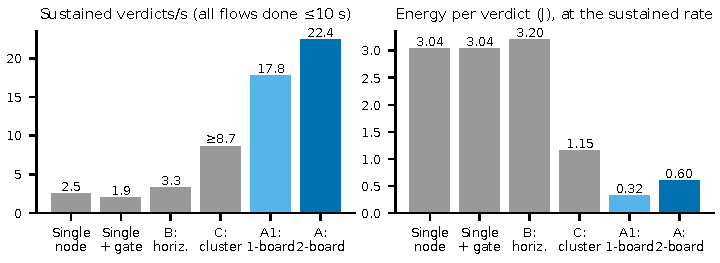
\includegraphics[width=\linewidth]{edge_capacity.pdf}\par}
  \vspace{3mm}
  \begin{itemize}
    \item The gate inside the classifier's process gains \bad{nothing}: each
          batch still waits for a PySpark call that costs seconds.
    \item The same split as two processes \key{on one board} (A1) already
          sustains \good{7×} the single node at 0.32\,J per verdict.
    \item A second board adds about a quarter more capacity at twice the
          energy per verdict: headroom, not efficiency.
  \end{itemize}
\end{sect}

\vfill
% ---------------------------------------------------------------------
\begin{sect}{Result 2 --- What the gate costs, end to end}
  \par\vspace{2mm}{\centering\tabsize
  \adjustbox{max width=\linewidth}{\begin{tabular*}{\linewidth}{@{\extracolsep{\fill}}l r r c c c@{}}
    \toprule
    Mode & Attacks & Missed: gate / clf & FP & Recall & F1 \\
    \midrule
    \textbf{A: full replay} & 1{,}518 & 463 / 0 & 0 & \bad{69.5\%} & 0.820 \\
    A1: split, one board & 882 & 278 / 0 & 0 & 68.5\% & 0.813 \\
    C: Spark cluster     & 381 & 115 / 0 & 0 & 69.8\% & 0.822 \\
    Single node + gate   & 200 & 55 / 0 & 0 & 72.5\% & 0.841 \\
    Gate off (single, B) & 242 & -- / 0 & 0 & 100\% & 1.000 \\
    \bottomrule
  \end{tabular*}}\par}\vspace{2.5mm}
  \vspace{3mm}
  \begin{minipage}[c]{0.56\linewidth}
    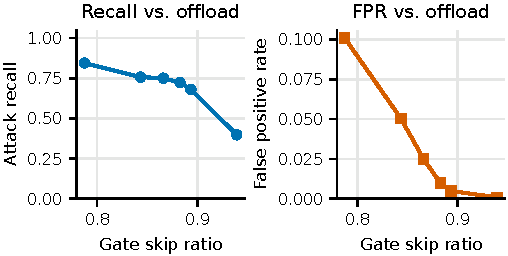
\includegraphics[width=\linewidth]{gate_operating_points.pdf}
  \end{minipage}\hfill
  \begin{minipage}[c]{0.42\linewidth}\raggedright
    \begin{itemize}
      \item \good{Precision 100\%}: no false alarm on 8{,}483 benign flows.
      \item All 463 misses were \bad{skipped by the gate}. The classifier
            made no error.
      \item A \key{tunable trade-off}: at quantile 0.995 the gate skips
            89.4\% of flows, forwards 68.1\% of attacks.
    \end{itemize}
  \end{minipage}
\end{sect}

\vfill
% ---------------------------------------------------------------------
\begin{sect}{Result 3 --- Another network: CSE-CIC-IDS2018}
  \par\vspace{2mm}{\centering\tabsize
  \adjustbox{max width=\linewidth}{\begin{tabular*}{\linewidth}{@{\extracolsep{\fill}}l c c@{}}
    \toprule
    Replayed flows (10{,}000 each, once) & CICIDS2017 & CSE-CIC-IDS2018 \\
    \midrule
    Flows forwarded by the gate   & 11.0\% & \bad{30.4\%} \\
    Sustained capacity (flows/s)  & 22.4   & \bad{≈8} \\
    Attack flows / detected       & 1{,}518 / 1{,}055 & 1{,}276 / \bad{10} \\
    Missed: by gate / by classifier & 463 / 0 & 712 / 554 \\
    End-to-end recall / F1        & 69.5\% / 0.820 & \bad{0.8\% / 0.016} \\
    Classifier alone, recall      & 99.8\% & 1.8\% \\
    \bottomrule
  \end{tabular*}}\par}\vspace{2.5mm}
  \vspace{3mm}
  Models trained on CICIDS2017, kept unchanged. The gate forwards three times
  as many flows, and the classifier itself misses almost every 2018 attack.
  Offline, 1\% labelled target flows restore F1 to \good{0.92} and \good{0.99}.
  \begin{takeaway}
    Neither detection \emph{nor capacity} transfers: a new network needs a
    \textbf{recalibrated gate} and a \textbf{retrained classifier}.
  \end{takeaway}
\end{sect}


\vfill
% ---------------------------------------------------------------------
\begin{sect}[colframe=hustRed, colbacktitle=hustRed]{Conclusion}
  \begin{itemize}
    \item \key{Decoupling} gate and classifier gives 7--9× capacity
          at lower energy per verdict. The price is \bad{recall}, set by the gate.
    \item One board running the split is the \good{most efficient} choice
          (17.8\,flows/s, 0.32\,J). A second board buys headroom.
    \item \textbf{Limitations:} a two-node lab cluster over Wi-Fi with
          replayed traffic, Kafka and databases on the host PC, an unused GPU,
          and untested evasive traffic.
    \item \textbf{Next:} ONNX/TensorRT serving, live-traffic validation,
          federated retraining under drift.
  \end{itemize}
\end{sect}
\end{minipage}%
\end{lrbox}%
\typeout{POSTER colL=\the\dimexpr\ht\colL+\dp\colL\relax\space colR=\the\dimexpr\ht\colR+\dp\colR\relax}%
% Zero-height holder: the page builder never sees the columns' depth, so it
% cannot push them to a second page. The log line above gives the real
% heights; top + max(colL, colR) must stay below the 1189 mm page.
\par\nointerlineskip\noindent\vbox to 0pt{\hbox{\hspace*{30mm}\usebox{\colL}\hspace{19mm}\usebox{\colR}}\vss}

\end{document}
